% ============================================================
% 电路基础实验 —— 实验五 集成运算放大器电路 预习报告
% ============================================================

\documentclass[12pt]{ctexart}

% --- 宏包 ---
\usepackage{graphicx}
\usepackage{amsmath}
\usepackage{amssymb}
\usepackage{float}
\usepackage{booktabs}
\usepackage{siunitx}
\usepackage{caption}
\usepackage{subcaption}
\usepackage{enumitem}

\sisetup{per-mode=symbol}

\graphicspath{{./figures/}}

\usepackage[left=2.5cm, right=2.5cm, top=2.5cm, bottom=2.5cm]{geometry}

\setlength{\jot}{6pt}
\linespread{1.5}
\setlist{nosep}

\begin{document}

% ==================== 封面 ====================
\thispagestyle{empty}

\begin{center}
    \LARGE\textbf{第5次实验\ 集成运算放大器电路预习报告}

    \vspace{1cm}
    \normalsize
    组名：第7组\quad 姓名：郭浩然\quad 学号：2024303980
\end{center}

\vspace{1cm}

% ==================== 正文 ====================

% (10) 实验目的
\section{实验目的}

\begin{enumerate}[label=\arabic*.]
    \item 学习集成运算放大器 LM324 的基本结构与各引脚功能。
    \item 理解双电源供电的必要性及其对运放电路输出范围的影响。
    \item 掌握反向比例放大器电路的工作原理与增益计算方法。
    \item 掌握含运放的有源积分电路的工作原理与波形变换特性。
    \item 通过 Multisim 仿真验证理论分析结果。
\end{enumerate}

% (80) 实验原理
\section{实验原理}

\subsection{LM324 集成运算放大器}

LM324 是一款四运放集成电路，采用 14 引脚双列直插（DIP-14）封装，内部包含 4 个独立的运算放大器。与实验 2、3 中使用的 LM317（三端可调稳压器，仅有输入、输出、调节 3 个引脚）不同，LM324 的 14 个引脚分配如表~\ref{tab:lm324-pins} 所示。

\begin{table}[H]
    \centering
    \caption{LM324 引脚功能}
    \label{tab:lm324-pins}
    \begin{tabular}{cll}
        \toprule
        引脚号 & 名称 & 功能 \\
        \midrule
        1  & 输出 1       & 第 1 个运放的输出端 \\
        2  & 反相输入 1   & 第 1 个运放的反相输入端（$-$） \\
        3  & 同相输入 1   & 第 1 个运放的同相输入端（$+$） \\
        4  & $V_{\mathrm{CC}}$ & 正电源 \\
        5  & 同相输入 2   & 第 2 个运放的同相输入端（$+$） \\
        6  & 反相输入 2   & 第 2 个运放的反相输入端（$-$） \\
        7  & 输出 2       & 第 2 个运放的输出端 \\
        8  & 输出 3       & 第 3 个运放的输出端 \\
        9  & 反相输入 3   & 第 3 个运放的反相输入端（$-$） \\
        10 & 同相输入 3   & 第 3 个运放的同相输入端（$+$） \\
        11 & $V_{\mathrm{EE}}$/GND & 负电源或接地 \\
        12 & 同相输入 4   & 第 4 个运放的同相输入端（$+$） \\
        13 & 反相输入 4   & 第 4 个运放的反相输入端（$-$） \\
        14 & 输出 4       & 第 4 个运放的输出端 \\
        \bottomrule
    \end{tabular}
\end{table}

LM324 的引脚分布如图~\ref{fig:lm324-pinout} 所示。

\begin{figure}[H]
    \centering
    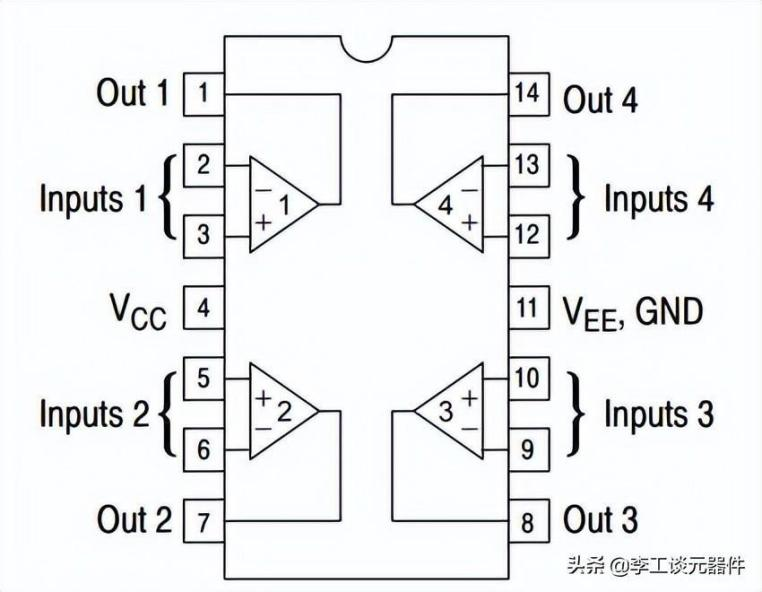
\includegraphics[width=0.48\textwidth]{lm324_pinout.jpeg}
    \caption{LM324 引脚分布图}
    \label{fig:lm324-pinout}
\end{figure}

LM324 的共模输入电压范围取决于供电电压，其上限约为 $V_{\mathrm{CC}}-\SI{1.5}{\volt}$，下限可达 $V_{\mathrm{EE}}$（含地电位）。当采用 $\pm\SI{5}{\volt}$ 双电源供电时，输入电压范围为
\begin{equation}
    \SI{-5}{\volt} \leqslant V_{\mathrm{CM}} \leqslant +\SI{3.5}{\volt}.
\end{equation}

\subsection{双电源供电}

为使集成运放 LM324 正常工作，需要提供正负对称的直流电源。以 $\pm\SI{5}{\volt}$ 双电源供电为例，即 $V_{\mathrm{CC}}=+\SI{5}{\volt}$，$V_{\mathrm{EE}}=-\SI{5}{\volt}$。双电源供电的意义在于：

\begin{enumerate}[label=(\arabic*)]
    \item \textbf{输出对称摆幅}：输出电压可在正、负方向对称摆动，能够完整放大交流信号的正、负半周，避免削顶失真。
    \item \textbf{简化偏置设计}：同相输入端可直接接地作为参考零电位，无需额外设计复杂的直流偏置网络。
    \item \textbf{扩大输入范围}：共模输入范围覆盖零电位及负电压区域，可直接处理地电位附近的信号。
\end{enumerate}

单电源供电（如 $V_{\mathrm{CC}}=\SI{5}{\volt}$，$V_{\mathrm{EE}}=\SI{0}{\volt}$）时，LM324 的输入共模范围虽然包含地电位，可以工作，但输出仅能在 $0$ 至 $V_{\mathrm{CC}}$ 之间摆动，无法直接放大包含负半周的交流信号。若要处理交流信号，需额外设计偏置电路将信号抬升至电源电压中点附近，电路设计更复杂且输出动态范围减半。因此，在线性放大交流信号的场合，优先采用双电源供电。

\subsection{反向比例放大器}

反向比例放大器的基本结构：信号经输入电阻 $R_1$ 接入运放反相输入端，反馈电阻 $R_f$ 连接在输出与反相输入端之间，同相输入端通过偏置电阻接地。

利用理想运放的虚短（$v_+ = v_-$）和虚断（$i_+ = i_- = 0$）条件进行分析。同相输入端接地，故
\begin{equation}
    v_+ = 0 \implies v_- = 0 \quad (\text{虚地}).
\end{equation}
在反相输入节点列 KCL 方程：
\begin{equation}
    \frac{v_i - v_-}{R_1} = \frac{v_- - v_o}{R_f},
\end{equation}
代入 $v_- = 0$，得
\begin{equation}
    \frac{v_i}{R_1} = -\frac{v_o}{R_f}.
\end{equation}
因此，电压增益为
\begin{equation}
    A_v = \frac{v_o}{v_i} = -\frac{R_f}{R_1}.
    \label{eq:inverting-gain}
\end{equation}

本实验 Multisim 仿真中取 $R_1=\SI{1}{\kilo\ohm}$，$R_f=\SI{10}{\kilo\ohm}$，故理论增益为
\begin{equation}
    A_v = -\frac{R_f}{R_1} = -\frac{\SI{10}{\kilo\ohm}}{\SI{1}{\kilo\ohm}} = -10.
\end{equation}
即输出信号幅值为输入的 10 倍，且相位反转 $180°$。

\subsection{有源积分电路}

将反向比例放大器中的反馈电阻 $R_f$ 替换为电容 $C$，即构成有源积分电路。

利用虚短和虚断条件，在反相输入节点列 KCL 方程：
\begin{equation}
    \frac{v_i}{R_1} = -C\frac{\mathrm{d}v_o}{\mathrm{d}t}.
\end{equation}
对两端积分，得
\begin{equation}
    v_o(t) = -\frac{1}{R_1 C}\int_0^t v_i(\tau)\,\mathrm{d}\tau + v_o(0).
    \label{eq:integrator}
\end{equation}

在频域中，传递函数为
\begin{equation}
    H(j\omega) = \frac{V_o}{V_i} = -\frac{1}{j\omega R_1 C}.
\end{equation}

本实验仿真中取 $R_1=\SI{1}{\kilo\ohm}$，$C_1=\SI{1}{\micro\farad}$，积分时间常数为
\begin{equation}
    R_1 C_1 = \SI{1}{\kilo\ohm}\times\SI{1}{\micro\farad} = \SI{1}{\milli\second}.
\end{equation}

当输入方波信号时，正半周 $v_i = V_m$（常数），积分后输出线性下降；负半周 $v_i = -V_m$，积分后输出线性上升。因此输出呈三角波，斜坡斜率为
\begin{equation}
    \left|\frac{\mathrm{d}v_o}{\mathrm{d}t}\right| = \frac{V_m}{R_1 C_1}.
\end{equation}

\subsection{Multisim 仿真}

\subsubsection{反向比例放大器仿真}

反向比例放大器的 Multisim 仿真电路如图~\ref{fig:inverting-amp} 所示。使用 LM324AD（U1A），$R_1=\SI{1}{\kilo\ohm}$，$R_f=\SI{10}{\kilo\ohm}$，偏置电阻 $R_2=\SI{1}{\kilo\ohm}$，双电源 $V_{\mathrm{CC}}=+\SI{5}{\volt}$，$V_{\mathrm{EE}}=-\SI{5}{\volt}$。函数发生器（XFG1）提供正弦波输入，示波器（XSC1）同时观测输入与输出波形。

\begin{figure}[H]
    \centering
    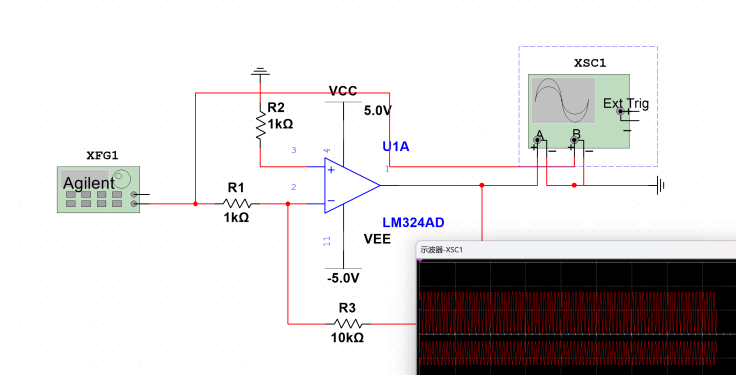
\includegraphics[width=0.82\textwidth]{inverting_amp_multisim.png}
    \caption{反向比例放大器 Multisim 仿真电路}
    \label{fig:inverting-amp}
\end{figure}

仿真预期：输出正弦波幅值为输入的 10 倍，相位反转 $180°$。

\subsubsection{有源积分电路仿真}

有源积分电路的 Multisim 仿真电路如图~\ref{fig:integrator} 所示。使用 LM324AD（U1A），$R_1=\SI{1}{\kilo\ohm}$，$C_1=\SI{1}{\micro\farad}$，双电源 $\pm\SI{5}{\volt}$。函数发生器输入方波信号，示波器观测输入方波与输出三角波。

\begin{figure}[H]
    \centering
    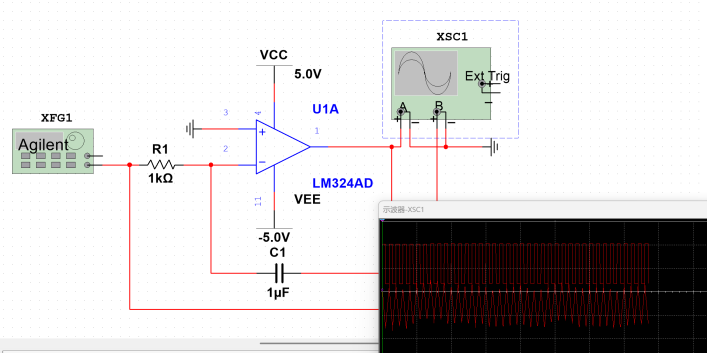
\includegraphics[width=0.82\textwidth]{integrator_multisim.png}
    \caption{有源积分电路 Multisim 仿真电路}
    \label{fig:integrator}
\end{figure}

仿真预期：方波输入下输出为三角波，斜率由积分时间常数 $R_1 C_1=\SI{1}{\milli\second}$ 决定。

\begin{table}[H]
    \centering
    \caption{集成运放电路仿真结果预期}
    \label{tab:simulation-expectation}
    \begin{tabular}{lll}
        \toprule
        电路 & 输入信号 & 理论预期输出 \\
        \midrule
        反向比例放大器 & 正弦波 & 幅值放大 10 倍，相位反转 $180°$ \\
        有源积分电路   & 方波   & 三角波，斜率 $V_m/(R_1 C_1)$ \\
        \bottomrule
    \end{tabular}
\end{table}

% (10) 实验器件
\section{实验器件}

\begin{itemize}
    \item 面包板 $\times 1$
    \item 直流稳压电源（双路输出）$\times 1$
    \item 函数信号发生器 RIGOL DG922 $\times 1$
    \item 示波器 RIGOL DHO1204 $\times 1$
    \item 数字万用表 RIGOL DM858 $\times 1$
    \item 集成运算放大器 LM324 $\times 1$
    \item 电阻：$\SI{1}{\kilo\ohm}\times 2$，$\SI{10}{\kilo\ohm}\times 1$
    \item 电容：$\SI{1}{\micro\farad}\times 1$
    \item 导线若干
\end{itemize}

\end{document}
